\section{Results and Discussion}
\label{sec:results}

\subsection{Fine-tuning: before and after}
\label{sec:res-ft}

Table~\ref{tab:main} compares the untuned Qwen2.5-1.5B-Instruct with the selected LoRA model on
identical validation and test examples, with the identical label-first prompt and greedy decoding.
Fine-tuning raises held-out test accuracy from 0.039 to \textbf{0.748}, macro-F1 from 0.077 to
\textbf{0.569} and evidence micro-F1 from 0.095 to \textbf{0.513}; every output of both models
was valid JSON with a valid label, so the gains are not a formatting artefact. The zero-shot model
is degenerate under this prompt: it answers \emph{excluded} for every validation exclusion criterion
and \emph{not applicable} for almost every inclusion criterion. With the evidence-first prompt the
same untuned model reaches 0.209 accuracy (macro-F1 0.142) on validation, still mostly answering
\emph{excluded}, i.e.\ confusing ``the note is about the excluded condition'' with ``the patient has
it''. The untuned model is thus highly prompt-sensitive, and asking it to cite evidence first helps
it, whereas after fine-tuning the answer order barely matters (Section~\ref{sec:res-abl}).

\begin{table}[t]
\centering
\caption{Before/after fine-tuning (label-first prompt, greedy). Ev.\ = evidence;
empty = agreement on records with no gold evidence.}
\label{tab:main}
\setlength{\tabcolsep}{3pt}
\begin{tabular}{llcccccc}
\toprule
 & & \multicolumn{2}{c}{Label} & \multicolumn{2}{c}{Ev.\ micro} & Ev.\ macro & Ev.\ \\
Split & Model & Acc & M-F1 & P & F1 & F1 & empty \\
\midrule
\multirow{2}{*}{Val} & zero-shot & 0.015 & 0.009 & 0.043 & 0.075 & 0.119 & 0.138 \\
 & LoRA & 0.743 & 0.544 & 0.504 & 0.551 & 0.606 & 0.836 \\
\midrule
\multirow{2}{*}{Test} & zero-shot & 0.039 & 0.077 & 0.054 & 0.095 & 0.138 & 0.207 \\
 & LoRA & \textbf{0.748} & \textbf{0.569} & 0.439 & \textbf{0.513} & 0.606 & 0.869 \\
\midrule
\multicolumn{8}{l}{\emph{Test by criterion type (LoRA)}} \\
 & inclusion & 0.773 & 0.417 & 0.466 & 0.582 & 0.686 & 0.633 \\
 & exclusion & 0.733 & 0.521 & 0.345 & 0.328 & 0.381 & 0.930 \\
\bottomrule
\end{tabular}
\end{table}

Fig.~\ref{fig:cm} and Table~\ref{tab:perclass} break the test result down. The model is reliable on
the frequent classes (F1 0.83--0.84 for \emph{included}, \emph{not excluded} and inclusion
\emph{not enough information}) and on exclusion \emph{not applicable} (precision 0.75). It never
predicts the rare inclusion classes: all seven \emph{not included} and all three \emph{not
applicable} inclusion cases are answered \emph{not enough information} (six) or \emph{included}
(one). Its weakest class is exclusion \emph{not enough information} (recall 0.07): 25 of 28 such
criteria are predicted \emph{not excluded}. Overall accuracy therefore overstates performance on
the decisions that matter most; macro-F1, which weighs every class equally, is the more honest
summary. Inclusion criteria have higher accuracy but lower macro-F1 than exclusion criteria
because the two zero-recall classes are both inclusion classes.

\begin{figure*}[t]
\centering
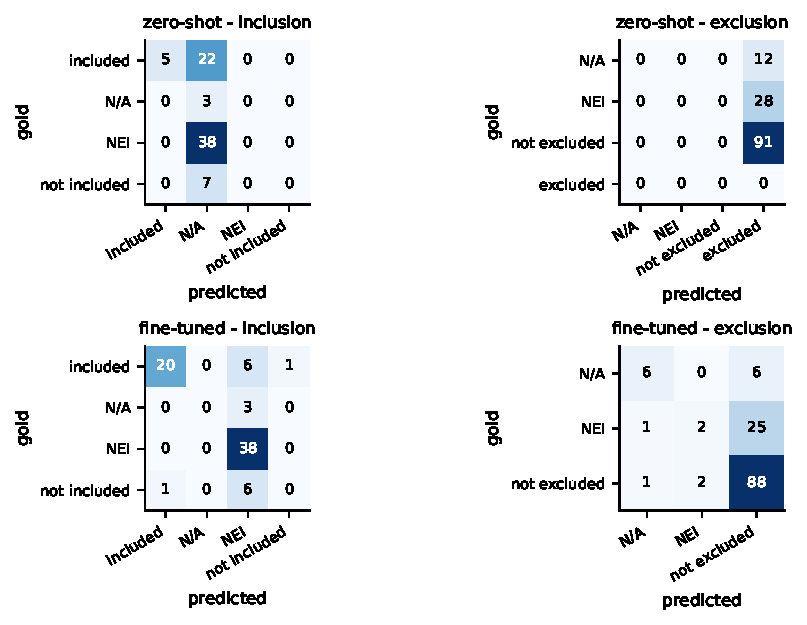
\includegraphics[width=0.8\textwidth]{figures/confusion_test}
\caption{Test confusion matrices (rows gold, columns predicted) for the zero-shot (top) and
fine-tuned (bottom) model, inclusion (left) and exclusion (right). The test split has no
\emph{excluded} example.}
\label{fig:cm}
\end{figure*}

\begin{table}[t]
\centering
\caption{Per-class test metrics of the final model.}
\label{tab:perclass}
\setlength{\tabcolsep}{4pt}
\begin{tabular}{llcccr}
\toprule
Type & Class & P & R & F1 & n \\
\midrule
\multirow{4}{*}{Inclusion} & included & 0.95 & 0.74 & 0.83 & 27 \\
 & not included & 0.00 & 0.00 & 0.00 & 7 \\
 & not enough information & 0.72 & 1.00 & 0.84 & 38 \\
 & not applicable & 0.00 & 0.00 & 0.00 & 3 \\
\midrule
\multirow{4}{*}{Exclusion} & excluded & -- & -- & -- & 0 \\
 & not excluded & 0.74 & 0.97 & 0.84 & 91 \\
 & not enough information & 0.50 & 0.07 & 0.13 & 28 \\
 & not applicable & 0.75 & 0.50 & 0.60 & 12 \\
\bottomrule
\end{tabular}
\end{table}

\textbf{Evidence.} When the gold evidence set is non-empty the model recovers 62\% of the gold
sentences (micro recall 0.617) at precision 0.44; per-record macro-F1 is 0.61. On the 145 test
records without gold evidence it correctly cites nothing in 87\% of cases. Evidence precision is
lowest for exclusion criteria (0.35), where the model tends to cite every symptom sentence of a
note when it judges a criterion. Even when the label is correct, the cited set differs from the
expert set in 36 of 154 correct predictions, often by citing one plausible extra sentence.

\textbf{Seed variability and reproducibility.} Retraining the final recipe with seeds 43 and 44
gives validation macro-F1 $0.554 \pm 0.008$ and test macro-F1 $0.551 \pm 0.017$ (mean $\pm$ s.d.\
over seeds 42--44; test accuracy $0.738 \pm 0.013$, evidence micro-F1 $0.544 \pm 0.036$), so the
reported model is representative rather than a lucky run. The published adapter, downloaded from
the Hugging Face Hub and run in fp32 on the laptop CPU, reproduced the Kaggle T4 fp16 outputs
character for character on 40 of 40 validation examples.

\subsection{Training dynamics and ablations}
\label{sec:res-abl}

Fig.~\ref{fig:curves} shows the training loss (answer tokens only) and validation macro-F1 per epoch
for all variants; Table~\ref{tab:ablation} summarizes them. Training loss falls by an order of
magnitude in the first epoch and keeps decreasing, while teacher-forced validation loss is flat
after epoch 1--2 (0.13--0.15), so longer training mainly sharpens already-learned outputs: five
epochs reach the best evidence F1 (0.577) but not a better macro-F1. Oversampling drives the
training loss down to $\approx$0.005 by memorizing the repeated rare examples, and its validation
macro-F1 peaks after one epoch and then declines, a textbook overfitting pattern. It does shift
recall towards minority classes (validation \emph{included} 23$\rightarrow$32 of 35, exclusion
\emph{not enough information} 7$\rightarrow$13 of 26) at the expense of \emph{not excluded}
(95$\rightarrow$82 of 101).

\begin{figure*}[t]
\centering
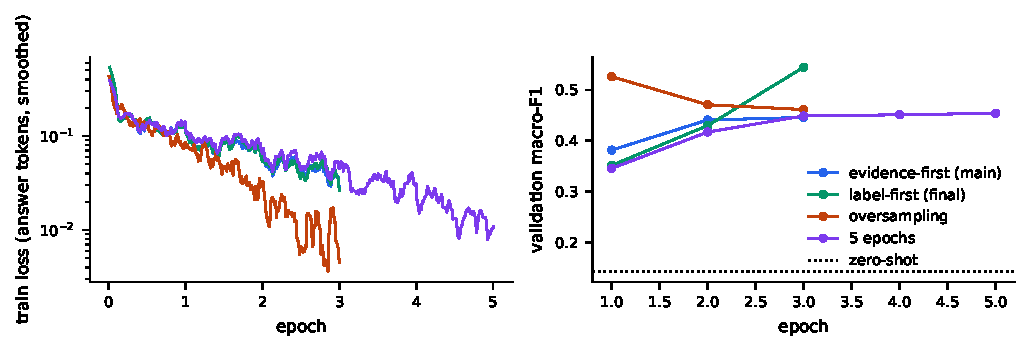
\includegraphics[width=0.85\textwidth]{figures/training_curves}
\caption{Left: training loss on answer tokens (moving average, log scale) per epoch. Right:
validation macro-F1 after each epoch; the dotted line is the evidence-first zero-shot baseline.}
\label{fig:curves}
\end{figure*}

\begin{table}[t]
\centering
\caption{Validation ablations (best epoch by validation macro-F1) and paired-bootstrap
difference in macro-F1 vs.\ the evidence-first main run (95\% interval).}
\label{tab:ablation}
\setlength{\tabcolsep}{2.5pt}
\begin{tabular}{lccccc}
\toprule
Variant (epoch) & Acc & M-F1 & Ev.\ F1 & $\Delta$M-F1 [95\% CI] & T4 s \\
\midrule
evidence-first (3) & 0.748 & 0.446 & 0.544 & -- & 810 \\
label-first (3) & 0.743 & \textbf{0.545} & 0.551 & +0.069 [$-$0.030, 0.168] & 822 \\
oversampling (1) & 0.738 & 0.526 & 0.489 & +0.063 [$-$0.031, 0.177] & 1290 \\
5 epochs (5) & 0.752 & 0.454 & 0.577 & +0.008 [$-$0.015, 0.033] & 1378 \\
\midrule
0.5B, label-first (2) & 0.748 & 0.447 & 0.486 & \multicolumn{2}{l}{(draft model)} \\
\bottomrule
\end{tabular}
\end{table}

No variant is reliably better than the main run: every bootstrap interval for accuracy, macro-F1
and evidence F1 contains zero, and oversampling lowers evidence F1 in 95\% of resamples. The
validation split contains only three \emph{not included}, two \emph{excluded} and one inclusion
\emph{not applicable} example, so a single extra correct rare-class prediction moves macro-F1 by
$\approx$0.1; label-first's lead is exactly one additional correct \emph{excluded}. We nevertheless
kept the selection rule fixed in advance (best validation macro-F1) and chose label-first, and the
seed study above shows that this configuration is stable. The fine-tuned 0.5B draft reaches 0.748
validation accuracy itself, which explains its high draft acceptance (Section~\ref{sec:res-spec}).

\subsection{Error analysis}
\label{sec:res-err}

The final model makes 52 label errors on the 206 test criteria. Table~\ref{tab:errors} lists
representative cases, grouped into the failure modes we observed.

\begin{table*}[t]
\centering
\caption{Representative test errors of the final model (annotation ID, criterion type; gold vs.\
predicted label with cited sentence IDs).}
\label{tab:errors}
\footnotesize
\setlength{\tabcolsep}{3pt}
\begin{tabular}{p{0.45cm}p{3.1cm}p{4.6cm}p{3.0cm}p{5.2cm}}
\toprule
ID & Criterion & Relevant note content & Gold $\rightarrow$ predicted & Failure mode \\
\midrule
186 & (I) Heart rate of at least 90/min & [2] ``\ldots tachypneic and tachycardic.'' & included [2] $\rightarrow$ NEI [3] & \emph{Under-inference}: qualitative term (tachycardic) not mapped to the numeric threshold. \\
187 & (I) Respiratory rate $\ge$ 20/min or \ldots & [2] same sentence & included [2] $\rightarrow$ NEI [2] & Cites the right sentence but refuses the inference. \\
382 & (I) $\ge$4 ACR criteria for SLE & [0--2] arthralgia, malar rash, alopecia, anemia, thrombocytopenia, ANA, anti-dsDNA & included [0,1,2] $\rightarrow$ NEI [0--3] & \emph{Multi-step reasoning}: requires counting criteria across sentences. \\
164 & (I) Surgical lower-limb revascularisation & [0] cardiac catheterization via the right femoral artery & not included $\rightarrow$ included [0,2] & \emph{Surface matching}: femoral/limb vocabulary taken as the procedure. \\
176 & (I) No history of central venous catheterization & [0] cardiac catheterization (arterial) & included [0] $\rightarrow$ not incl.\ [\,] & \emph{Negation and concept confusion}; decisive label with no evidence (\emph{unsupported}). \\
836 & (I) Episodic wheezing after age 6 or asthma & [0] 4-year-old; [1] ``no history of wheezing'' & not included [0,1] $\rightarrow$ NEI [0--7] & Age constraint and negation missed; over-citation of all 8 sentences. \\
389--412 & (E) e.g.\ severe renal impairment; IV cyclophosphamide; drug abuse & not mentioned & NEI [\,] $\rightarrow$ not excluded [\,] & \emph{Missing information treated as absence} (14 cases, one patient). \\
320 & (E) Heart failure or EF $<$30\% & not mentioned & not excluded [\,] $\rightarrow$ NEI [\,] & \emph{Contradictory annotation}: same situation as 389--412, opposite gold label. \\
771 & (E) Females of childbearing potential & [0] 5-year-old boy & N/A [0] $\rightarrow$ not excluded [\,] & Applicability: the model did not reason from sex/age. \\
322 & (E) Pregnant women / no contraception & [0] 48-year-old male & not excluded [0] $\rightarrow$ N/A [\,] & Contradictory annotation of the same situation as 771. \\
385 & (I) Ability to take oral medication & [4] boilerplate ``will comply with the trial protocol'' & included [4] $\rightarrow$ NEI [\,] & Dataset artefact sentence not used as evidence. \\
\bottomrule
\end{tabular}
\end{table*}

\textbf{Missing information versus absence.} The largest error group (25 of 52) is exclusion
criteria that the note never mentions, labelled \emph{not enough information} by the expert but
\emph{not excluded} by the model. This is the failure the task definition warns against, but the
training data itself is ambivalent: across the dataset, 365 of the 483 \emph{not excluded} labels
cite no evidence, i.e.\ annotators very often treated an unmentioned exclusion condition as absent.
Fourteen of the 25 errors come from a single test patient whose annotator consistently chose
\emph{not enough information} (IDs 389--412), while cases such as ID~320 show the opposite
convention within the same test split. The model learned the majority convention. Because of this,
the application never presents an evidence-free \emph{not excluded} as established: it is flagged
\emph{inferred from absence} and listed for verification (Section~\ref{sec:app}).

\textbf{Unsupported predictions.} 104 decisive predictions cite no sentence; 103 are \emph{not
excluded} (75 of them correct under the gold labels, reflecting the convention above) and one is the
wrong \emph{not included} of ID~176. A decisive label without evidence is flagged \emph{unsupported}
by the application.

\textbf{Conservatism on inclusion criteria.} Most inclusion errors go towards \emph{not enough
information} (15 of 17): the model rarely commits to \emph{not included} or \emph{not applicable}
and, as IDs 186/187 show, does not draw clinical inferences that the expert drew. Its errors are
therefore mostly ``safe'' (deferring to a clinician), but they lower recall of exactly the
exclusionary decisions a screening tool should surface.

\subsection{KV-cached decoding}
\label{sec:res-kv}

\textbf{Correctness.} On CPU in fp32 our forward pass matches the library's logits within $10^{-3}$
with each attention backend, chunked prefill through the cache equals a single full pass, and
cached, uncached and library greedy decoding produce identical tokens for three prompt/output
lengths (8, 24 and 40 new tokens); cache rollback restores the exact state (automated tests). On the
T4 in fp16 (Table~\ref{tab:kv}), cached decoding and library greedy agree in all 12 configurations,
and cached and uncached agree in 9 of the 11 configurations in which the uncached path was run; the two mismatches occur with the 294-token prompt at 64
and 128 new tokens.

We investigated this case by decoding step by step with both paths and recording the logits.
In fp32 the largest logit difference between the paths over 128 steps is $3.1\cdot10^{-4}$ while the
smallest top-2 margin is $2.8\cdot10^{-3}$, nine times larger, so no argmax can flip. In fp16 the
paths differ by up to 0.20 in a logit (fp16 has a resolution of $\approx$0.016 at logit magnitudes
around 20, and the paths use different matrix shapes and therefore different cuBLAS kernels), and
along this trajectory the top two candidates are at one step \emph{exactly tied} in fp16. Whether
such a tie is resolved identically depends on the kernel chosen, which is why the re-run did not
diverge while the benchmark run did. The mismatch is thus a precision effect, not a cache error.

\begin{table}[t]
\centering
\caption{KV-cached vs.\ uncached greedy decoding (T4, fp16, batch 1, median of 3 runs).
Mem = peak GPU memory in GiB (weights 2.88\,GiB); tok/s = new tokens / total time.}
\label{tab:kv}
\setlength{\tabcolsep}{2.5pt}
\begin{tabular}{rrcccccc}
\toprule
 & & \multicolumn{3}{c}{Cached} & \multicolumn{2}{c}{Uncached} & \\
Prompt & New & Prefill & tok/s & Mem & tok/s & Mem & Same \\
\midrule
294 & 16 & 0.056\,s & 32.3 & 3.91 & 12.6 & 4.01 & yes \\
294 & 128 & 0.058\,s & 34.1 & 3.92 & 12.1 & 4.08 & fp16 tie \\
384 & 128 & 0.062\,s & 34.0 & 3.95 & 9.9 & 4.13 & yes \\
1024 & 64 & 0.195\,s & 31.6 & 4.15 & 4.3 & 4.48 & yes \\
1024 & 128 & 0.193\,s & 33.1 & 4.16 & 4.2 & 4.52 & yes \\
2048 & 16 & 0.413\,s & 19.0 & 4.52 & 2.2 & 5.11 & yes \\
2048 & 64 & 0.410\,s & 28.6 & 4.52 & 2.2 & 5.14 & yes \\
\bottomrule
\end{tabular}
\end{table}

\textbf{Performance.} Fig.~\ref{fig:kv} and Table~\ref{tab:kv} show the expected asymptotics. With
the cache, each decode step processes one token, so throughput stays at 31--34 tokens/s for
prompts up to 1,024 tokens and the total time is almost independent of the prompt length; only the
prefill grows (0.06\,s at 294 tokens, 0.41\,s at 2,048). Without the cache every step reprocesses
the whole sequence, so throughput falls from 12.6 to 2.2 tokens/s and the speed-up of caching grows
from 2.6$\times$ to 13$\times$ (2.24\,s vs.\ 29.2\,s for 2,048 + 64 tokens). Caching also lowers peak
memory (4.52 vs.\ 5.14\,GiB at 2,048 tokens): the cache itself costs only 28\,KB per token
(56\,MiB for 2,048 tokens), whereas recomputation materializes the activations and attention
scores of the full sequence at every step. Our decoder is 21--37\% faster than library
\code{generate} in these runs (e.g.\ 3.76\,s vs.\ 4.81\,s for 294 + 128 tokens), mostly because it
skips the library's generality (logits processors, stopping criteria, cache abstractions).

\begin{figure*}[t]
\centering
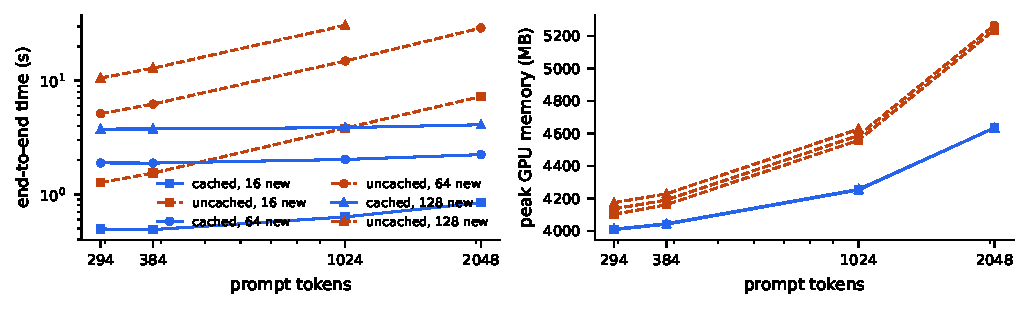
\includegraphics[width=0.85\textwidth]{figures/kv_cache}
\caption{KV-cached (solid) vs.\ uncached (dashed) greedy decoding on a T4: end-to-end time (left,
log-log) and peak GPU memory (right) as functions of prompt length for 16/64/128 new tokens.}
\label{fig:kv}
\end{figure*}

On the laptop CPU (fp32) the fine-tuned model needs about 12\,s per criterion in the application,
17\,s for the first criterion of a patient; prefix reuse saves the 234 shared prompt tokens
(of $\approx$360) for every subsequent criterion.

\subsection{Tiled attention}
\label{sec:res-attn}

\textbf{Correctness.} Against a float64 reference, both tiled variants (block 64 and 128) agree
with the reference and with PyTorch SDPA to within the precision of the input dtype on five shapes
including decode-style ($L_q{=}1$) and verification-style ($L_q{=}7$, $L_k{=}512$) causal cases:
maximum absolute error $9.8\cdot10^{-7}$ in fp32 and $1.6\cdot10^{-3}$ in fp16, with mean errors of
$4\cdot10^{-8}$ and $1.3\cdot10^{-4}$ (all implementations, including SDPA, show the same fp16 error,
which is the rounding of the fp16 output). In float64 the 64 unit tests agree with SDPA to
$10^{-10}$ for block sizes from 1 to 64, non-multiple lengths and padding masks. Used as the
attention backend of the real model, the tiled kernel reproduces the library's logits within
$2.6\cdot10^{-5}$ and identical generated tokens.

\textbf{Performance.} Fig.~\ref{fig:attn} shows the trade-off on the T4 (B=1, 12 heads, head
dimension 128, causal, fp16). Peak extra memory of the reference grows quadratically to 2.3\,GB at
4,096 tokens (the fp32 score matrix), while the tiled variants need 14--17\,MB, comparable to fused
SDPA (12\,MB): tiling achieves its purpose. Runtime tells the opposite story: tiled attention is
1.6--13$\times$ slower than our own reference and 65$\times$ slower than SDPA at 4,096 tokens
(254\,ms vs.\ 75\,ms vs.\ 3.9\,ms). The reason is that our tiling lives in Python: each of the
$(L/B)^2/2$ block pairs launches several small CUDA kernels (matrix products, exponentials,
rescaling) whose launch overhead dominates their arithmetic, every intermediate tile round-trips
through global memory, and larger blocks (128 vs.\ 64) are faster precisely because they launch fewer
kernels. A fused kernel such as FlashAttention performs the same online-softmax recurrence inside one
kernel, keeping tiles in on-chip shared memory and registers, so it gets the memory saving
\emph{and} the speed. The educational implementation demonstrates the algorithm and its memory
behaviour, not the speed.

\begin{figure*}[t]
\centering
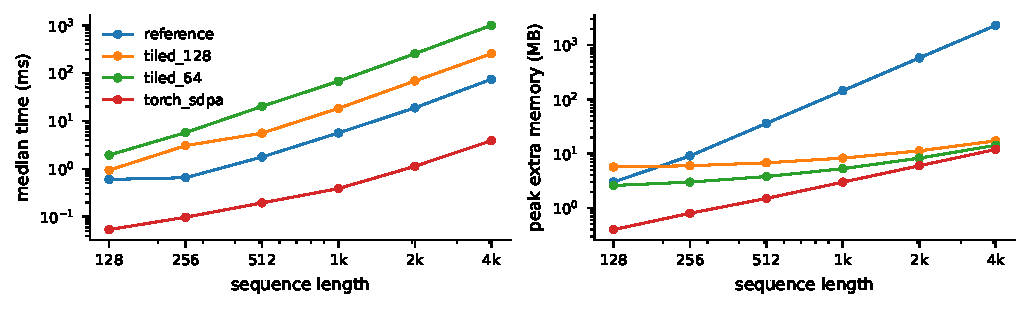
\includegraphics[width=0.85\textwidth]{figures/attention_perf}
\caption{Attention kernels on a T4 (fp16, B=1, H=12, d=128, causal): median runtime (left) and
peak extra GPU memory (right) vs.\ sequence length, both log scale.}
\label{fig:attn}
\end{figure*}

\subsection{Speculative decoding}
\label{sec:res-spec}

\textbf{Correctness.} Speculative decoding produced exactly the target's greedy tokens in all 96
benchmark configurations (two drafts $\times$ four draft lengths $\times$ 12 prompt/output lengths) and
on all 40 real screening prompts for both drafts. The unit tests additionally check equality for
$k\in\{1,3,5\}$ with a perfect draft, a noisy draft and a draft so noisy that fewer than half of
its tokens are accepted, which exercises the rejection and cache-rollback path, and stopping at EOS.

\textbf{Acceptance and speed.} Fine-tuning the draft on the same task raises acceptance on screening
prompts from 75.7\% to 92.6\% ($k=4$), and over longer generations from 61--84\% to 72--90\%
(Fig.~\ref{fig:spec}). Despite this, speculative decoding is not faster on the T4: on the 40
screening prompts it runs at 0.75$\times$ (base draft) and 0.90$\times$ (fine-tuned draft) of the
speed of KV-cached greedy, and over the length grid the speed-up ranges from 0.51 (base draft, $k=8$, short prompt) to 1.06.
With 128 new tokens and $k=4$, the fine-tuned draft gives 26.4--31.4 tokens/s against 31.2--34.2
for KV-cached greedy.

\textbf{Memory.} Speculative decoding keeps both models resident: 2.88\,GiB of fp16 target weights
plus 0.92\,GiB for the draft. In the benchmark both were loaded for every mode, so the measured peak
difference is the draft's own KV cache plus the activations of verifying $k{+}1$ tokens at once:
peak memory rises from 3.92 to 4.00\,GiB at a 294-token prompt and from 4.52 to 5.12\,GiB at 2,048
tokens ($k=4$, 128 new tokens). On the CPU-only laptop, where the models run in fp32, the draft adds
about 2\,GB, which is why the application checks free memory before loading it.

The explanation is the cost of a draft step relative to a target step. We measured single-token
decode steps of 23.6\,ms for the 0.5B draft and 28.5\,ms for the 1.5B target, a ratio $c=0.84$,
although the draft has a third of the parameters. At batch size 1 both models are dominated by
per-layer overhead (our decoder issues roughly 25 kernel launches per layer from Python, and the
draft has 24 layers against the target's 28) rather than by arithmetic or memory traffic. With
acceptance rate $\alpha$ and draft length $k$, the expected speed-up of
Leviathan et~al.~\cite{leviathan2023fast} is
$\frac{1-\alpha^{k+1}}{(1-\alpha)(ck+1)}$; with $c=0.84$ it predicts 1.05, 1.00 and 0.89 for
$\alpha=0.93$ and $k=2, 4, 8$, and 0.70 for $\alpha=0.75$, $k=4$, matching the measured 0.90 and
0.75 on screening prompts. Short outputs make things worse: a screening answer has only
$\approx$15 tokens, so the fixed cost of prefilling the draft model is amortized over very few
tokens. Speculative decoding pays off when $c$ is small, e.g.\ with a fused inference engine, a much
smaller draft relative to the target (a 7B target with a 0.5B draft) or memory-bound larger
batches, none of which applies to this deployment.

\begin{figure*}[t]
\centering
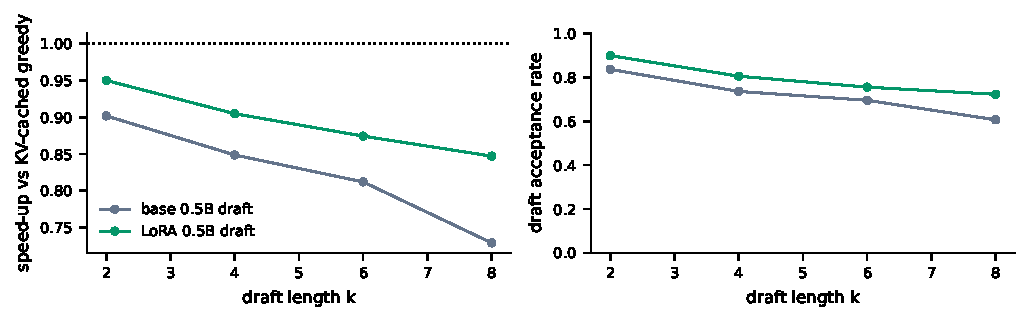
\includegraphics[width=0.85\textwidth]{figures/speculative}
\caption{Speculative decoding on a T4 with the base and the fine-tuned 0.5B draft, averaged over
the four prompt lengths at 128 new tokens: speed-up vs.\ KV-cached greedy (left; $<1$ is a
slowdown) and draft acceptance rate (right) as functions of the draft length $k$.}
\label{fig:spec}
\end{figure*}

\subsection{Application}
\label{sec:res-app}

Fig.~\ref{fig:app} shows the application screening a validation patient. Each criterion result
links its label to the highlighted note sentences, shows the evidence-only explanation and flags,
and the expert label when an example from the validation split is loaded. The benchmark page runs
the four decoding implementations on the current prompt and reports their timings, token equality
and acceptance; invalid inputs (empty note, empty or malformed criteria, prompts over the token
limit, unknown modes, malformed NCT IDs) are rejected with specific messages, and a failing criterion
does not abort the rest of a screening. Saved reports carry the model, adapter, decoding settings and
creation time.

\begin{figure*}[t]
\centering
\begin{minipage}[t]{0.49\textwidth}\vspace{0pt}
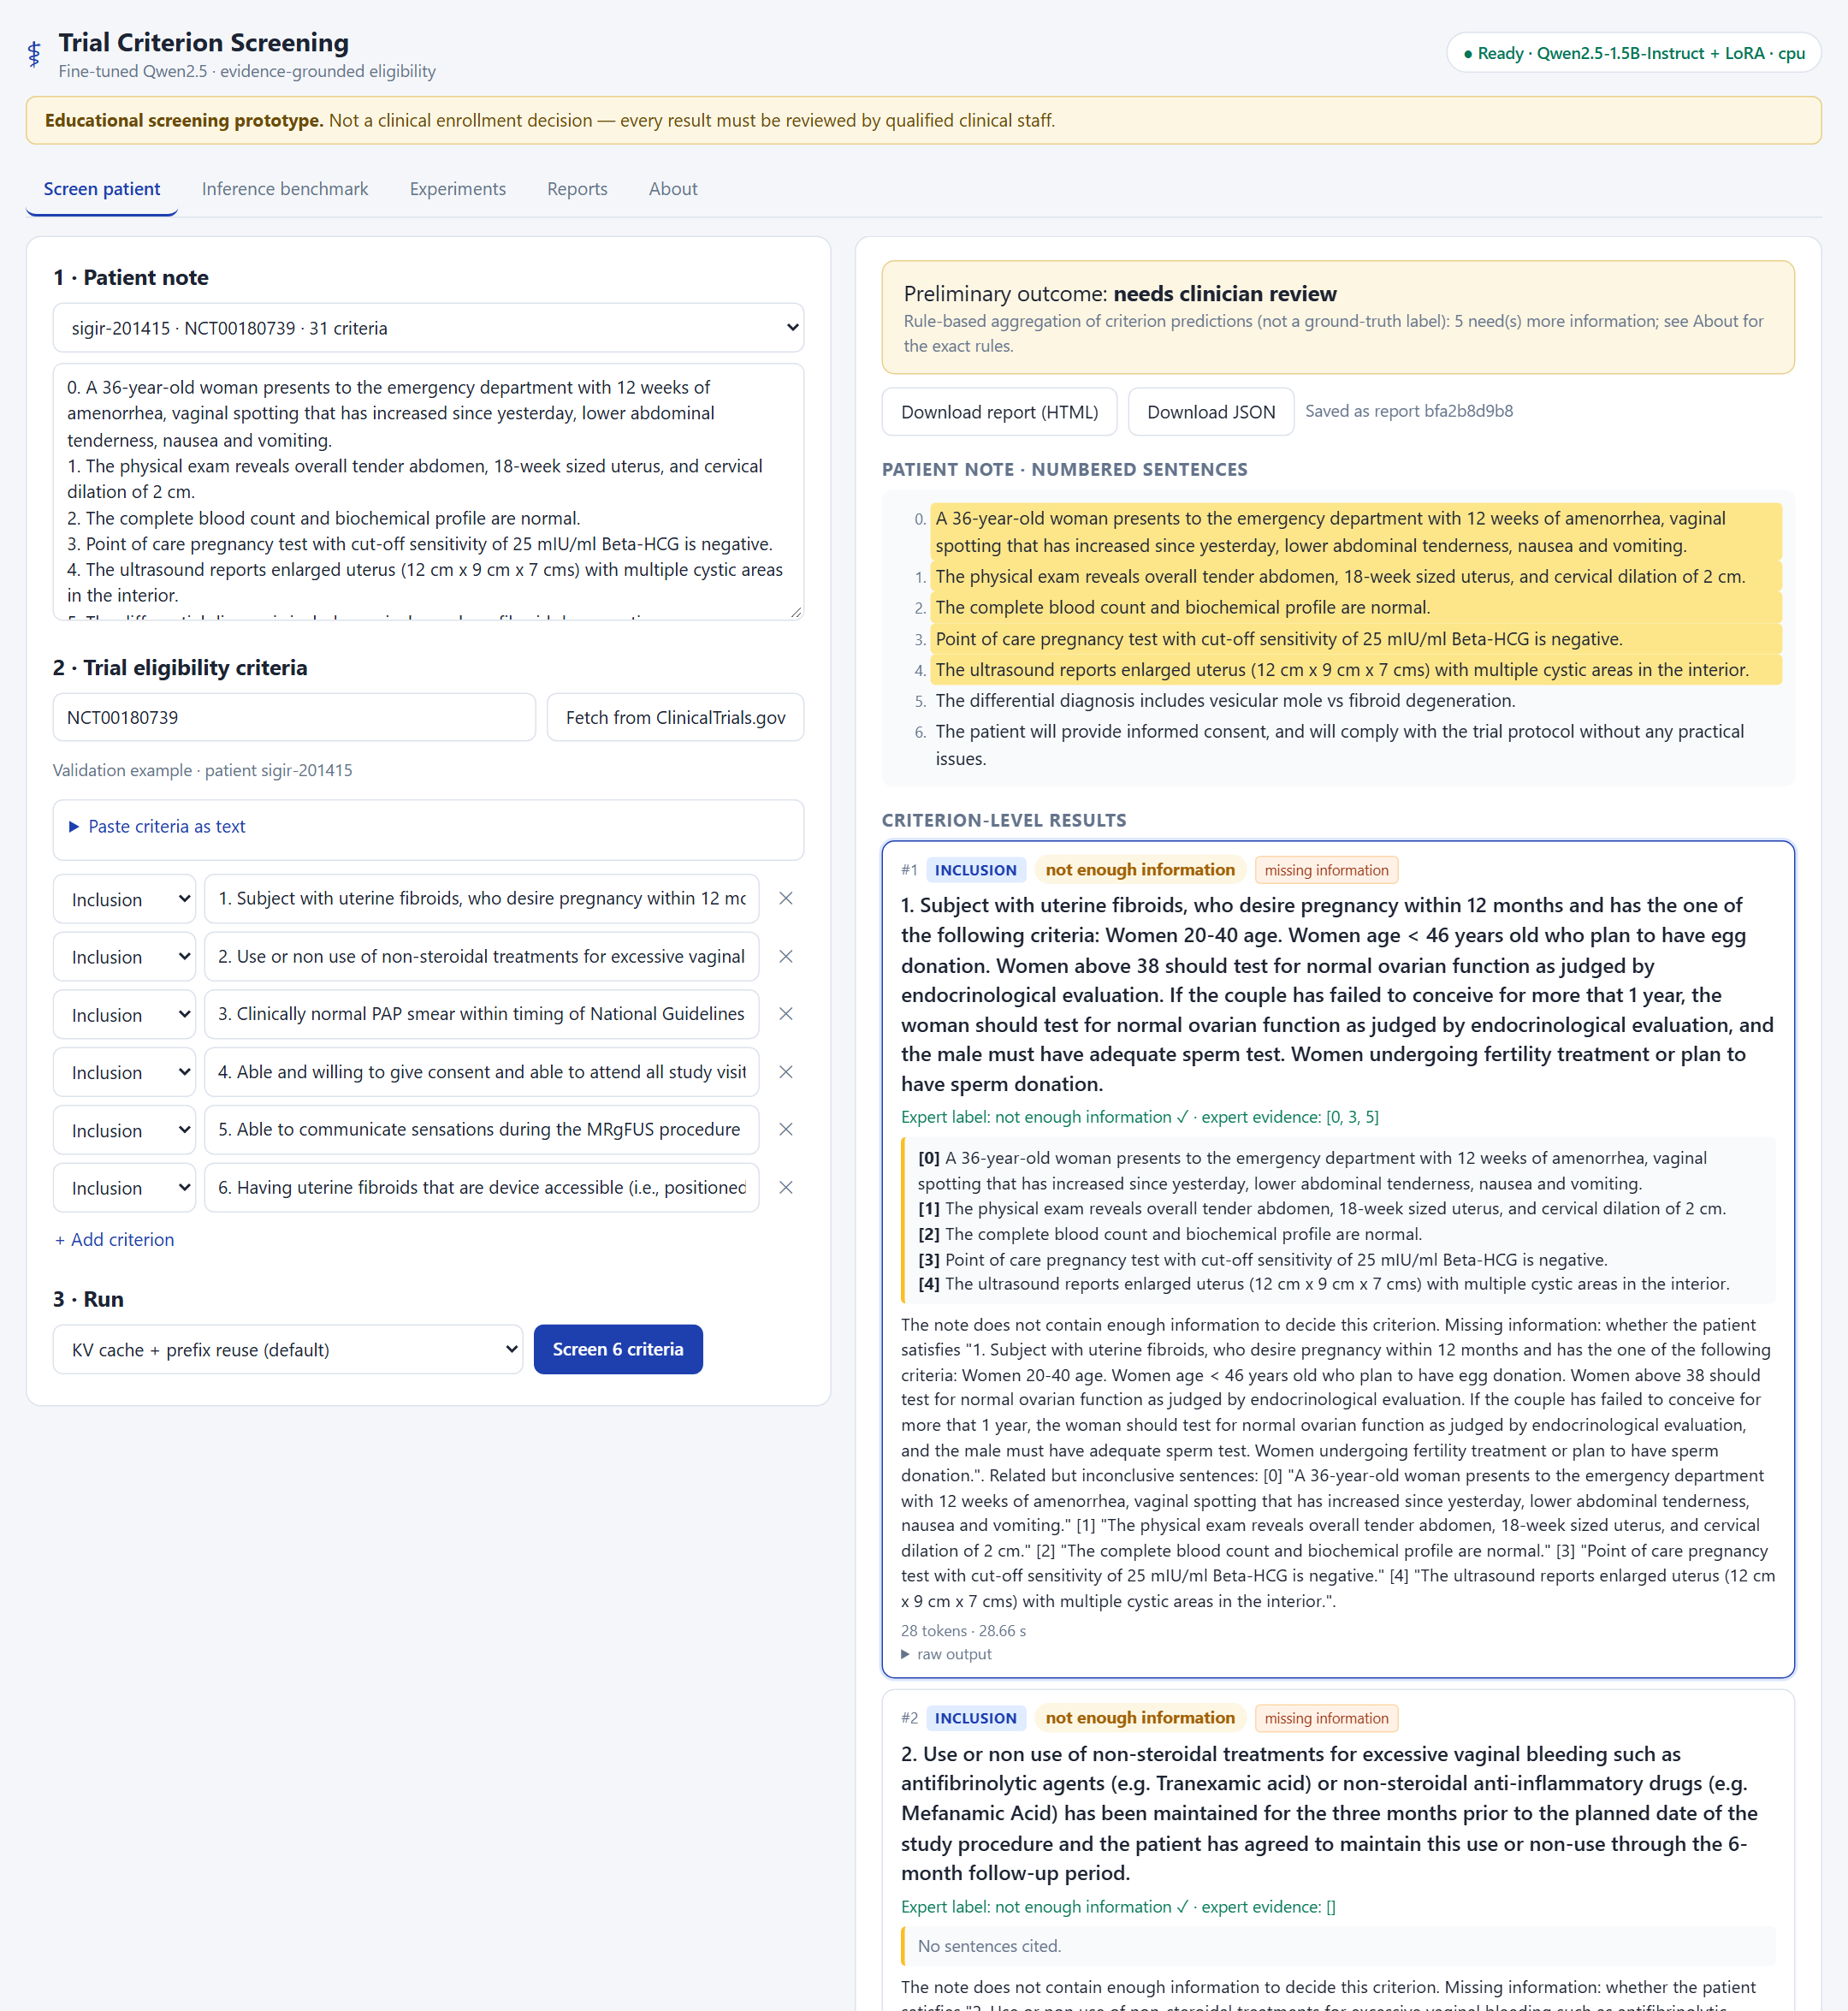
\includegraphics[width=\linewidth]{figures/screens/screen_top}
\end{minipage}\hfill
\begin{minipage}[t]{0.49\textwidth}\vspace{0pt}
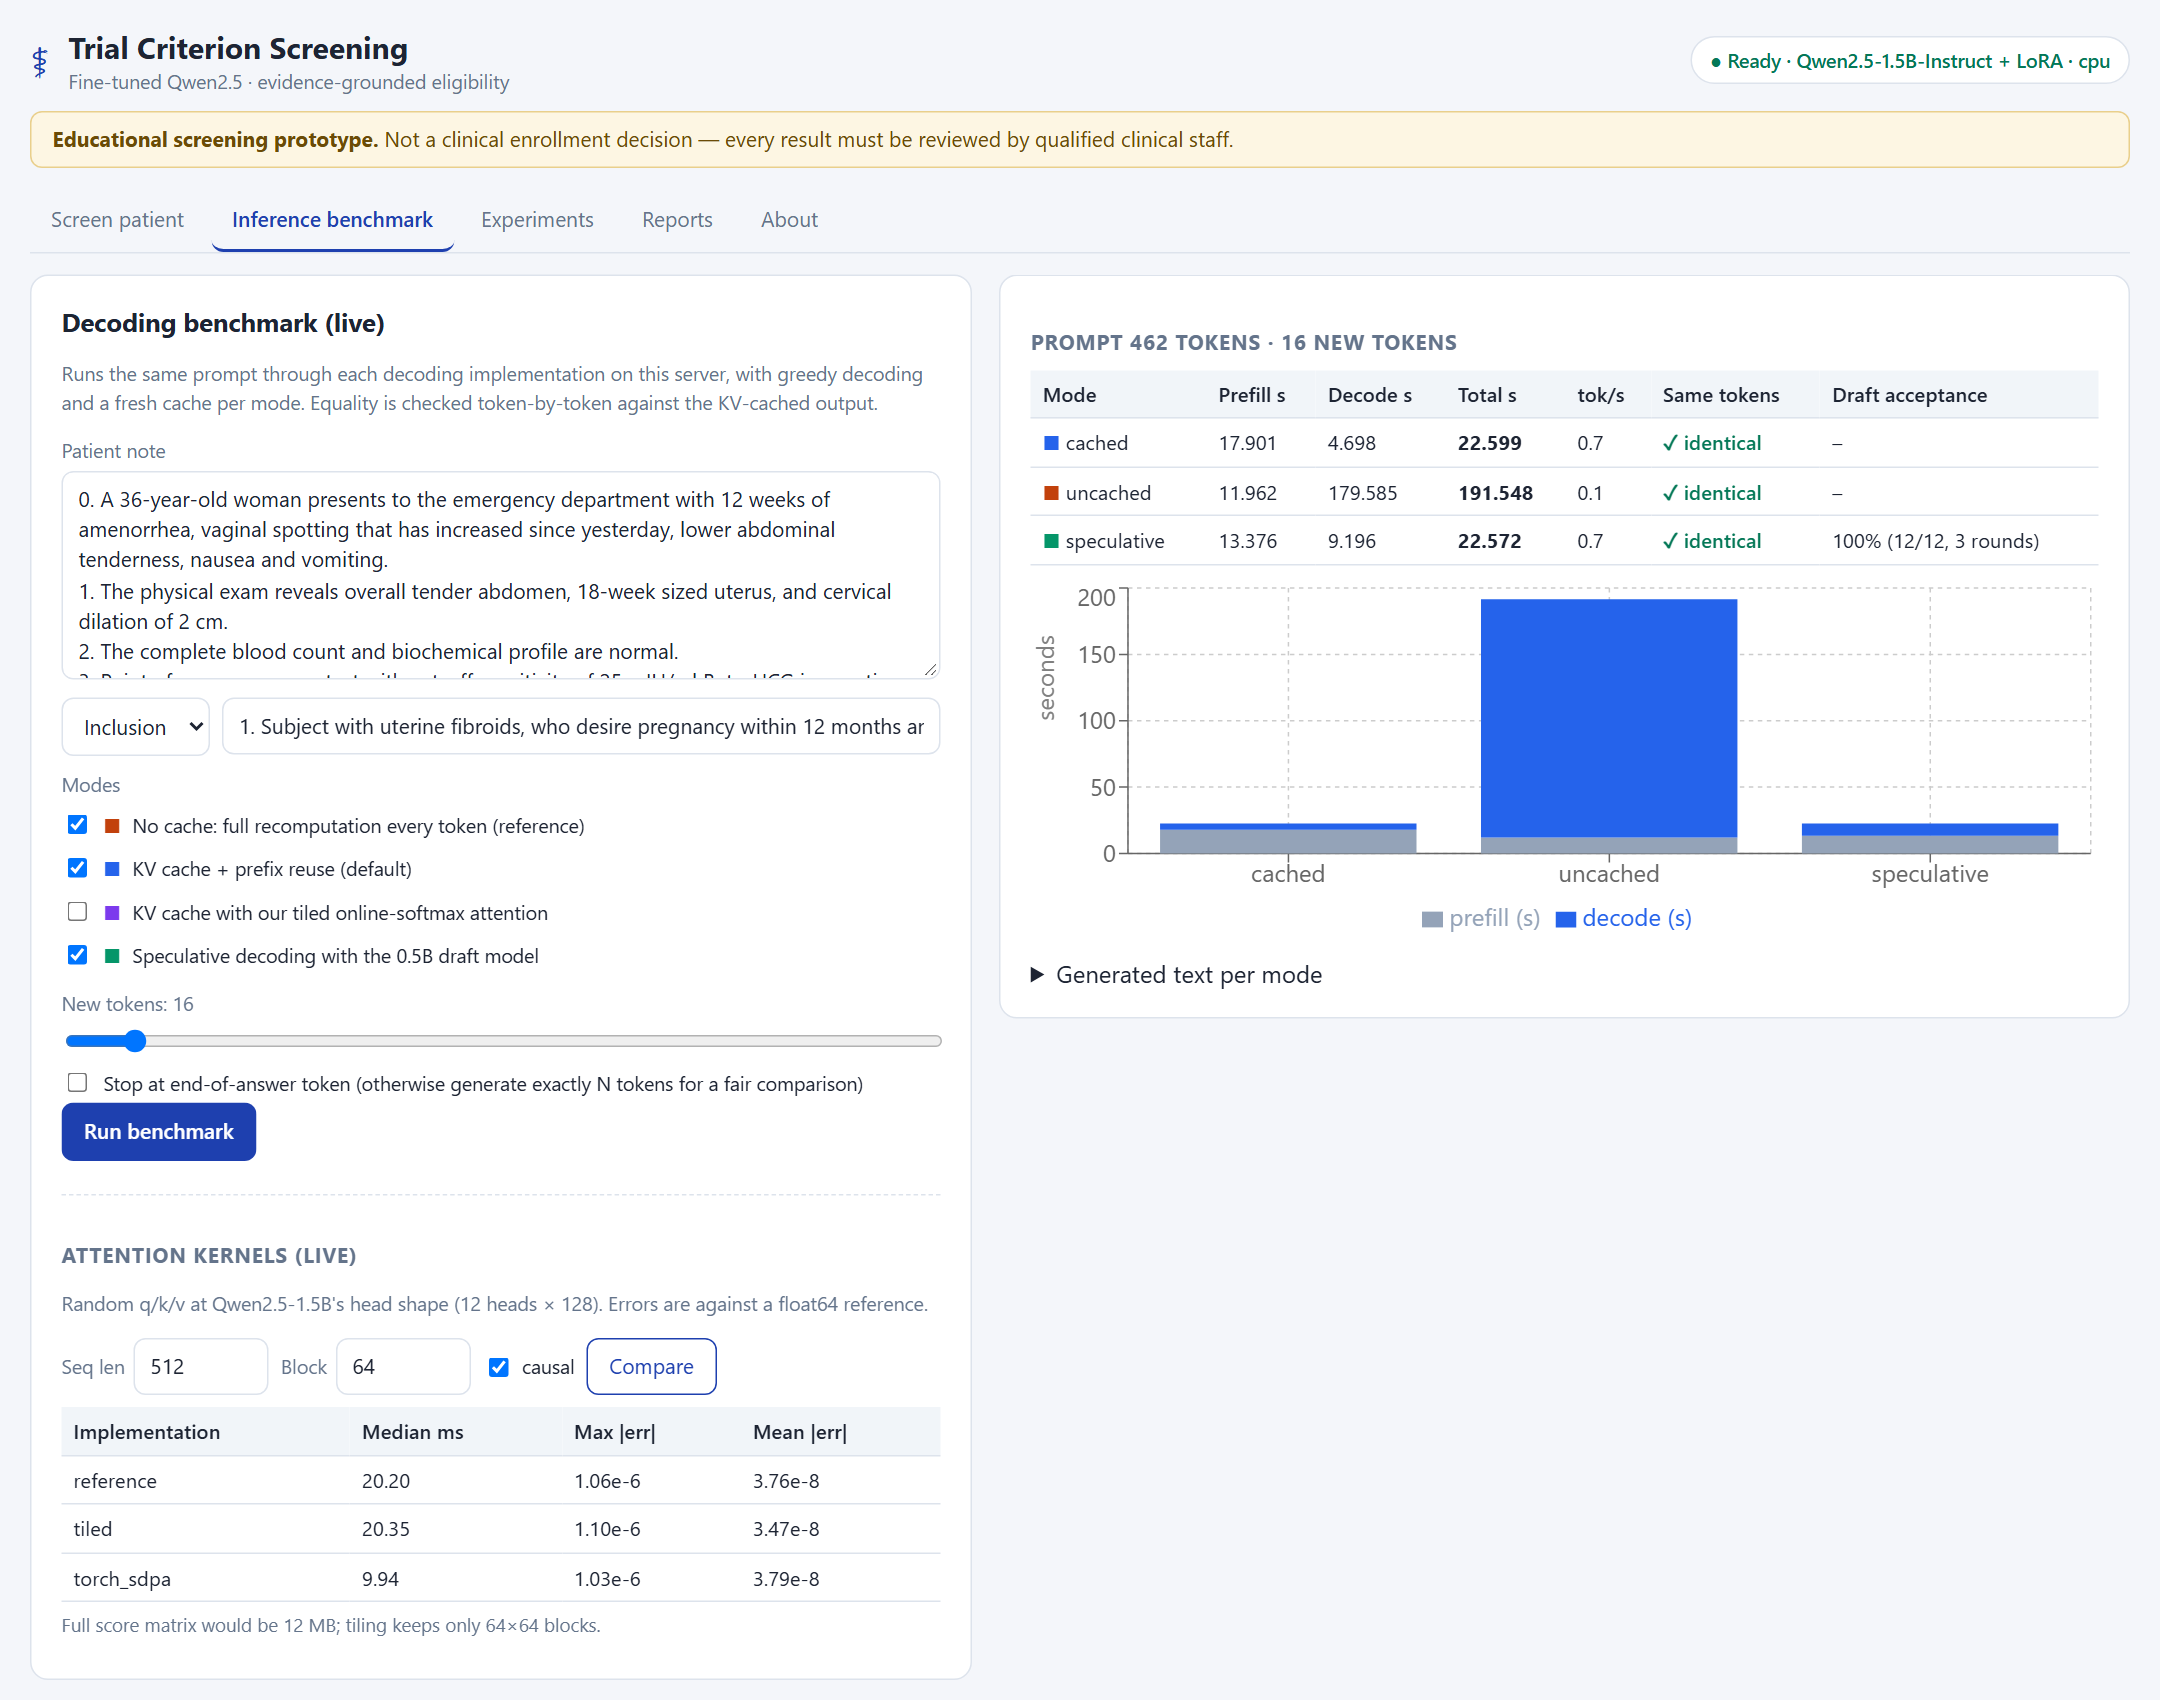
\includegraphics[width=\linewidth]{figures/screens/benchmark_crop}
\end{minipage}
\caption{The application running in Docker on the CPU-only laptop with the published adapter. Left:
screening six criteria of a validation patient; the selected result's cited sentences are highlighted
in the numbered note, the explanation quotes them, and the expert label is shown for comparison
(all six match). Right: the live benchmark page comparing KV-cached, uncached and speculative
decoding on the same prompt (identical tokens, 100\% draft acceptance; uncached decoding is
8.5$\times$ slower), and the live attention-kernel accuracy check.}
\label{fig:app}
\end{figure*}
